%!TeX root=../wowtop.tex

\ArtChapter[What I Saw of the Destruction of Weybridge and Shepperton]{12head}


\lettrine[lines=4]{A}{s} the dawn grew brighter we withdrew from the window from which we had watched the Martians, and went very quietly downstairs.

\zz
The artilleryman agreed with me that the house was no place to stay in. He proposed, he said, to make his way Londonward, and thence rejoin his battery—№ 12, of the Horse Artillery. My plan was to return at once to Leatherhead; and so greatly had the strength of the Martians impressed me that I had determined to take my wife to Newhaven, and go with her out of the country forthwith. For I already perceived clearly that the country about London must inevitably be the scene of a disastrous struggle before such creatures as these could be destroyed.

Between us and Leatherhead, however, lay the third cylinder, with its guarding giants. Had I been alone, I think I should have taken my chance and struck across country. But the artilleryman dissuaded me: »It's no kindness to the right sort of wife,« he said, »to make her a widow«; and in the end I agreed to go with him, under cover of the woods, northward as far as Street Cobham before I parted with him. Thence I would make a big detour by Epsom to reach Leatherhead.

I should have started at once, but my companion had been in active service and he knew better than that. He made me ransack the house for a flask, which he filled with whisky; and we lined every available pocket with packets of biscuits and slices of meat. Then we crept out of the house, and ran as quickly as we could down the ill-made road by which I had come overnight. The houses seemed deserted. In the road lay a group of three charred bodies close together, struck dead by the Heat-Ray; and here and there were things that people had dropped—a clock, a slipper, a silver spoon, and the like poor valuables. At the corner turning up towards the post office a little cart, filled with boxes and furniture, and horseless, heeled over on a broken wheel. A cash box had been hastily smashed open and thrown under the debris.

Except the lodge at the Orphanage, which was still on fire, none of the houses had suffered very greatly here. The Heat-Ray had shaved the chimney tops and passed. Yet, save ourselves, there did not seem to be a living soul on Maybury Hill. The majority of the inhabitants had escaped, I suppose, by way of the Old Woking road—the road I had taken when I drove to Leatherhead—or they had hidden.
\makeatletter
\@ifclasswith{scrbook}{a5paper}
{%

}{%
\begin{wrapfigure}{O}{0.5\textwidth}
\centering
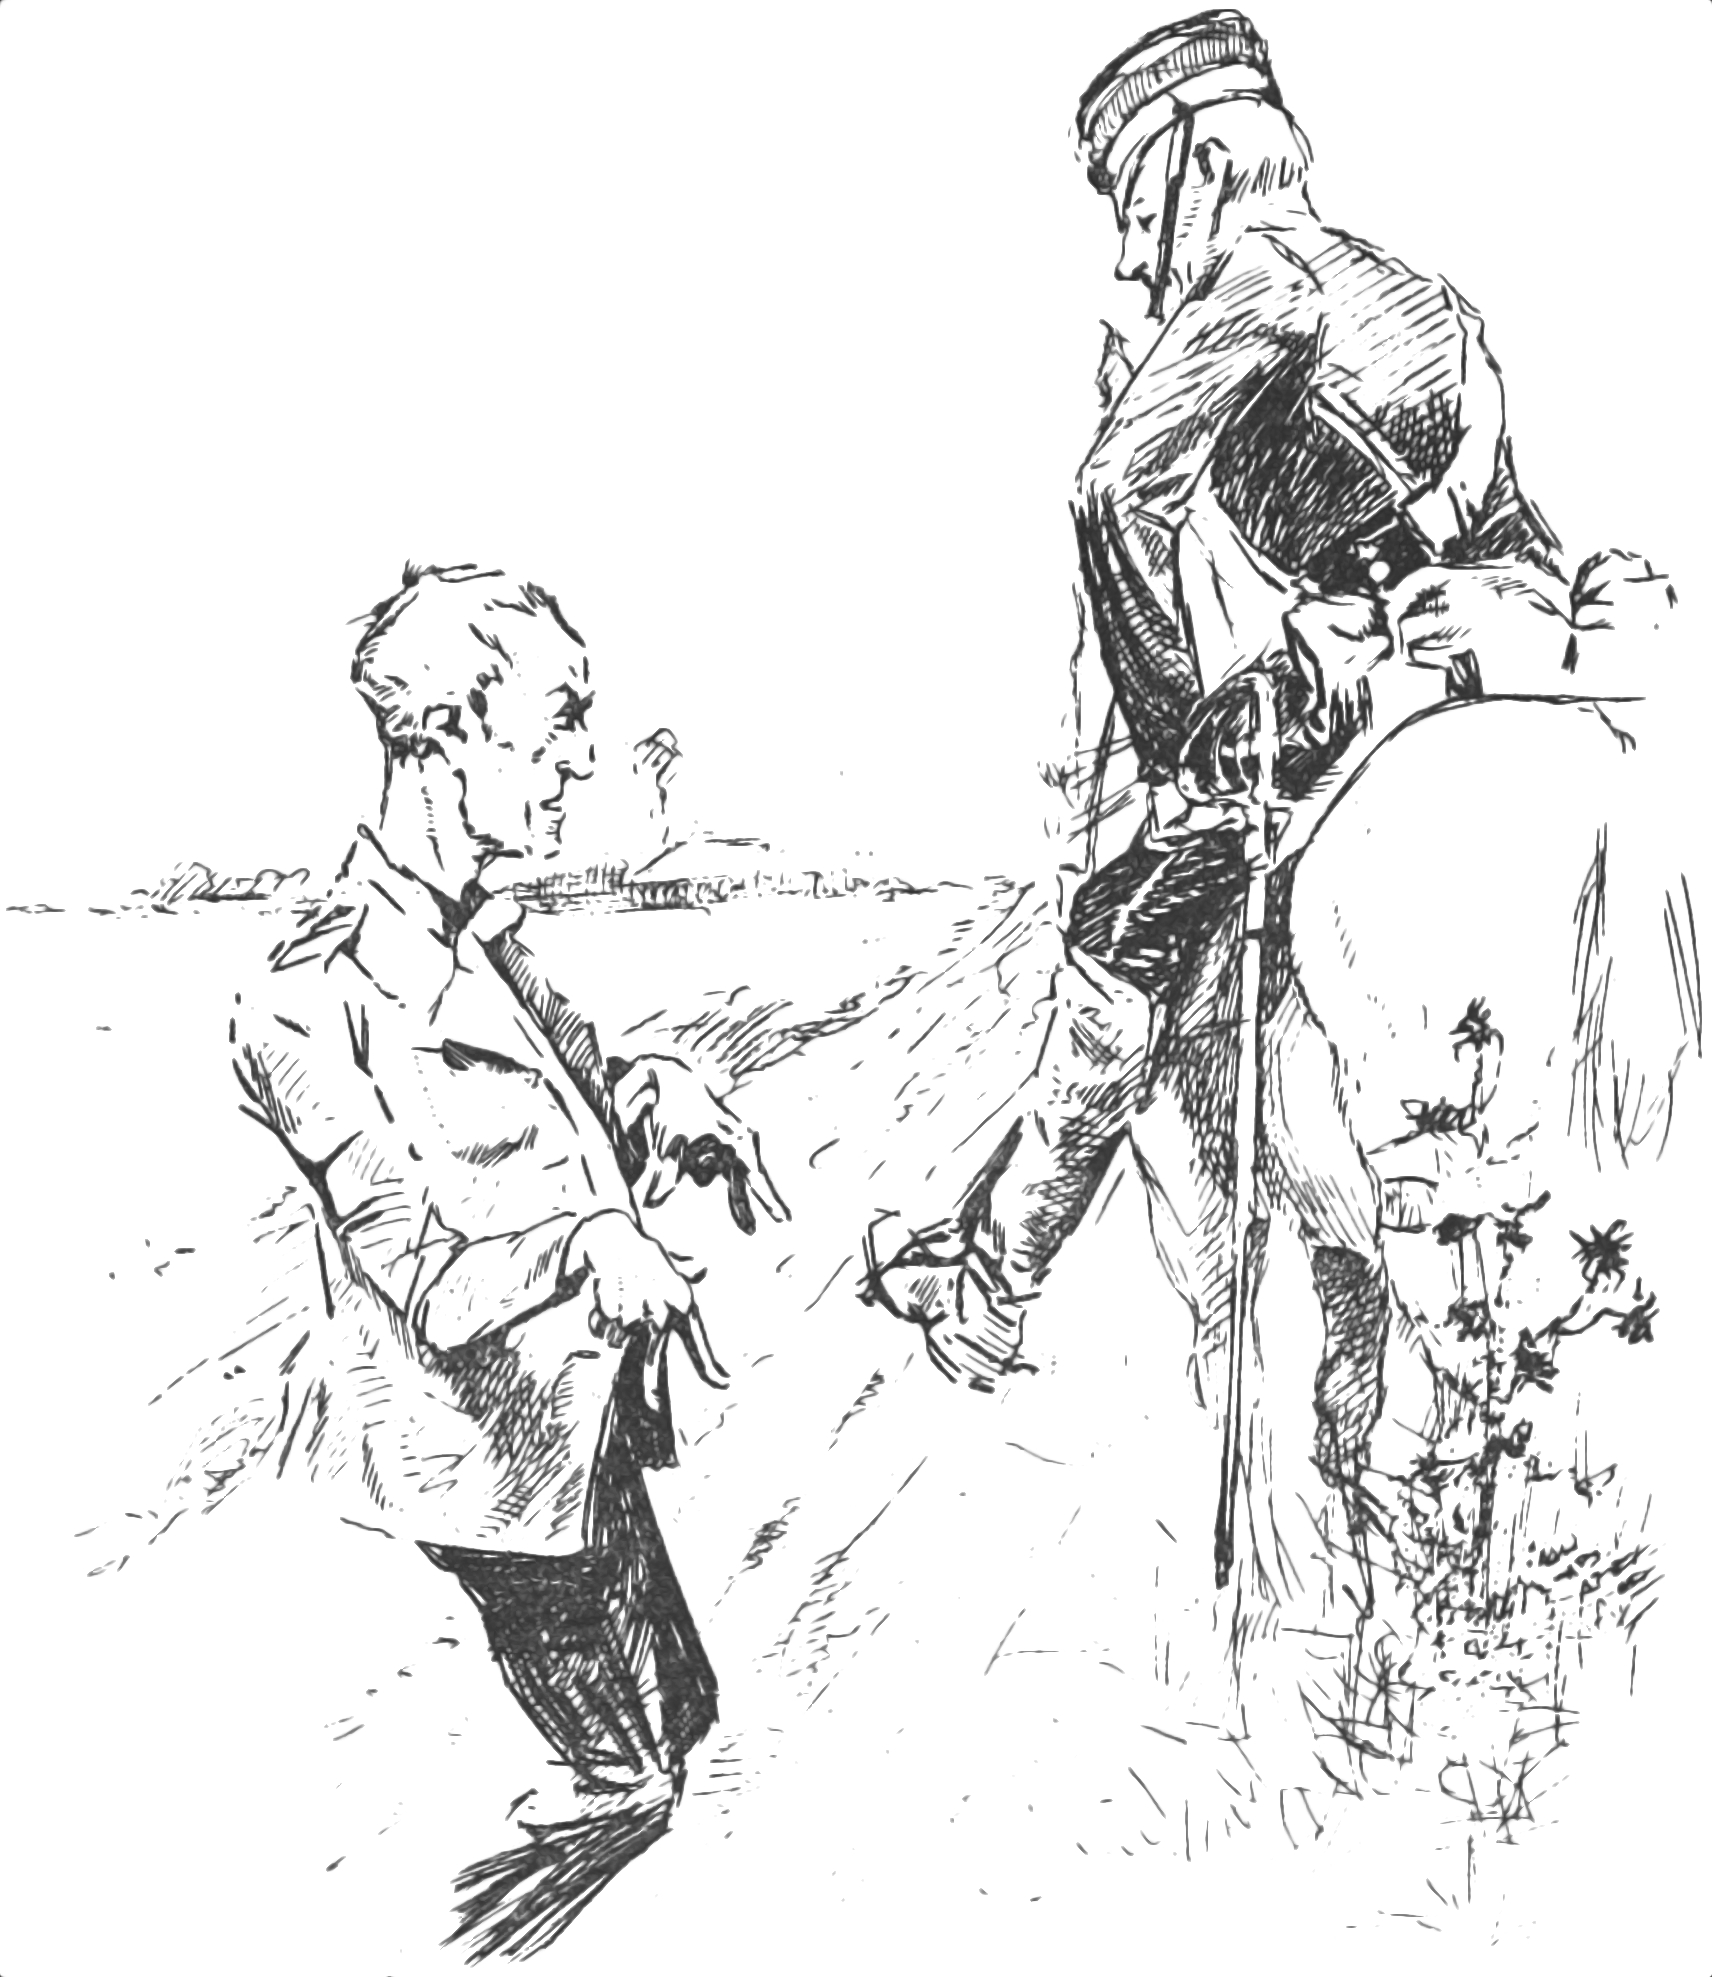
\includegraphics[width=0.5\textwidth]{12inspection}
\end{wrapfigure}
}
\makeatother


We went down the lane, by the body of the man in black, sodden now from the overnight hail, and broke into the woods at the foot of the hill. We pushed through these towards the railway without meeting a soul. The woods across the line were but the scarred and blackened ruins of woods; for the most part the trees had fallen, but a certain proportion still stood, dismal grey stems, with dark brown foliage instead of green.

On our side the fire had done no more than scorch the nearer trees; it had failed to secure its footing. In one place the woodmen had been at work on Saturday; trees, felled and freshly trimmed, lay in a clearing, with heaps of sawdust by the sawing-machine and its engine. Hard by was a temporary hut, deserted. There was not a breath of wind this morning, and everything was strangely still. Even the birds were hushed, and as we hurried along I and the artilleryman talked in whispers and looked now and again over our shoulders. Once or twice we stopped to listen.



After a time we drew near the road, and as we did so we heard the clatter of hoofs and saw through the tree stems three cavalry soldiers riding slowly towards Woking. We hailed them, and they halted while we hurried towards them. It was a lieutenant and a couple of privates of the 8\textsuperscript{th} Hussars, with a stand like a theodolite, which the artilleryman told me was a heliograph.

»You are the first men I've seen coming this way this morning,« said the lieutenant. »What's brewing?«

His voice and face were eager. The men behind him stared curiously. The artilleryman jumped down the bank into the road and saluted.

»Gun destroyed last night, sir. Have been hiding. Trying to rejoin battery, sir. You'll come in sight of the Martians, I expect, about half a mile along this road.«

»What the dickens are they like?« asked the lieutenant.

»Giants in armour, sir. Hundred feet high. Three legs and a body like `luminium, with a mighty great head in a hood, sir.«

»Get out!« said the lieutenant. »What confounded nonsense!«

»You'll see, sir. They carry a kind of box, sir, that shoots fire and strikes you dead.«

»What d'ye mean—a gun?«

»No, sir,« and the artilleryman began a vivid account of the Heat-Ray. Halfway through, the lieutenant interrupted him and looked up at me. I was still standing on the bank by the side of the road.

»It's perfectly true,« I said.

»Well,« said the lieutenant, »I suppose it's my business to see it too. Look here«—to the artilleryman—»we're detailed here clearing people out of their houses. You'd better go along and report yourself to Brigadier-General Marvin, and tell him all you know. He's at Weybridge. Know the way?«

»I do,« I said; and he turned his horse southward again.

»Half a mile, you say?« said he.

»At most,« I answered, and pointed over the treetops southward. He thanked me and rode on, and we saw them no more.

\makeatletter
\@ifclasswith{scrbook}{a5paper}
{%
\begin{wrapfigure}{O}{0.5\textwidth}
\centering
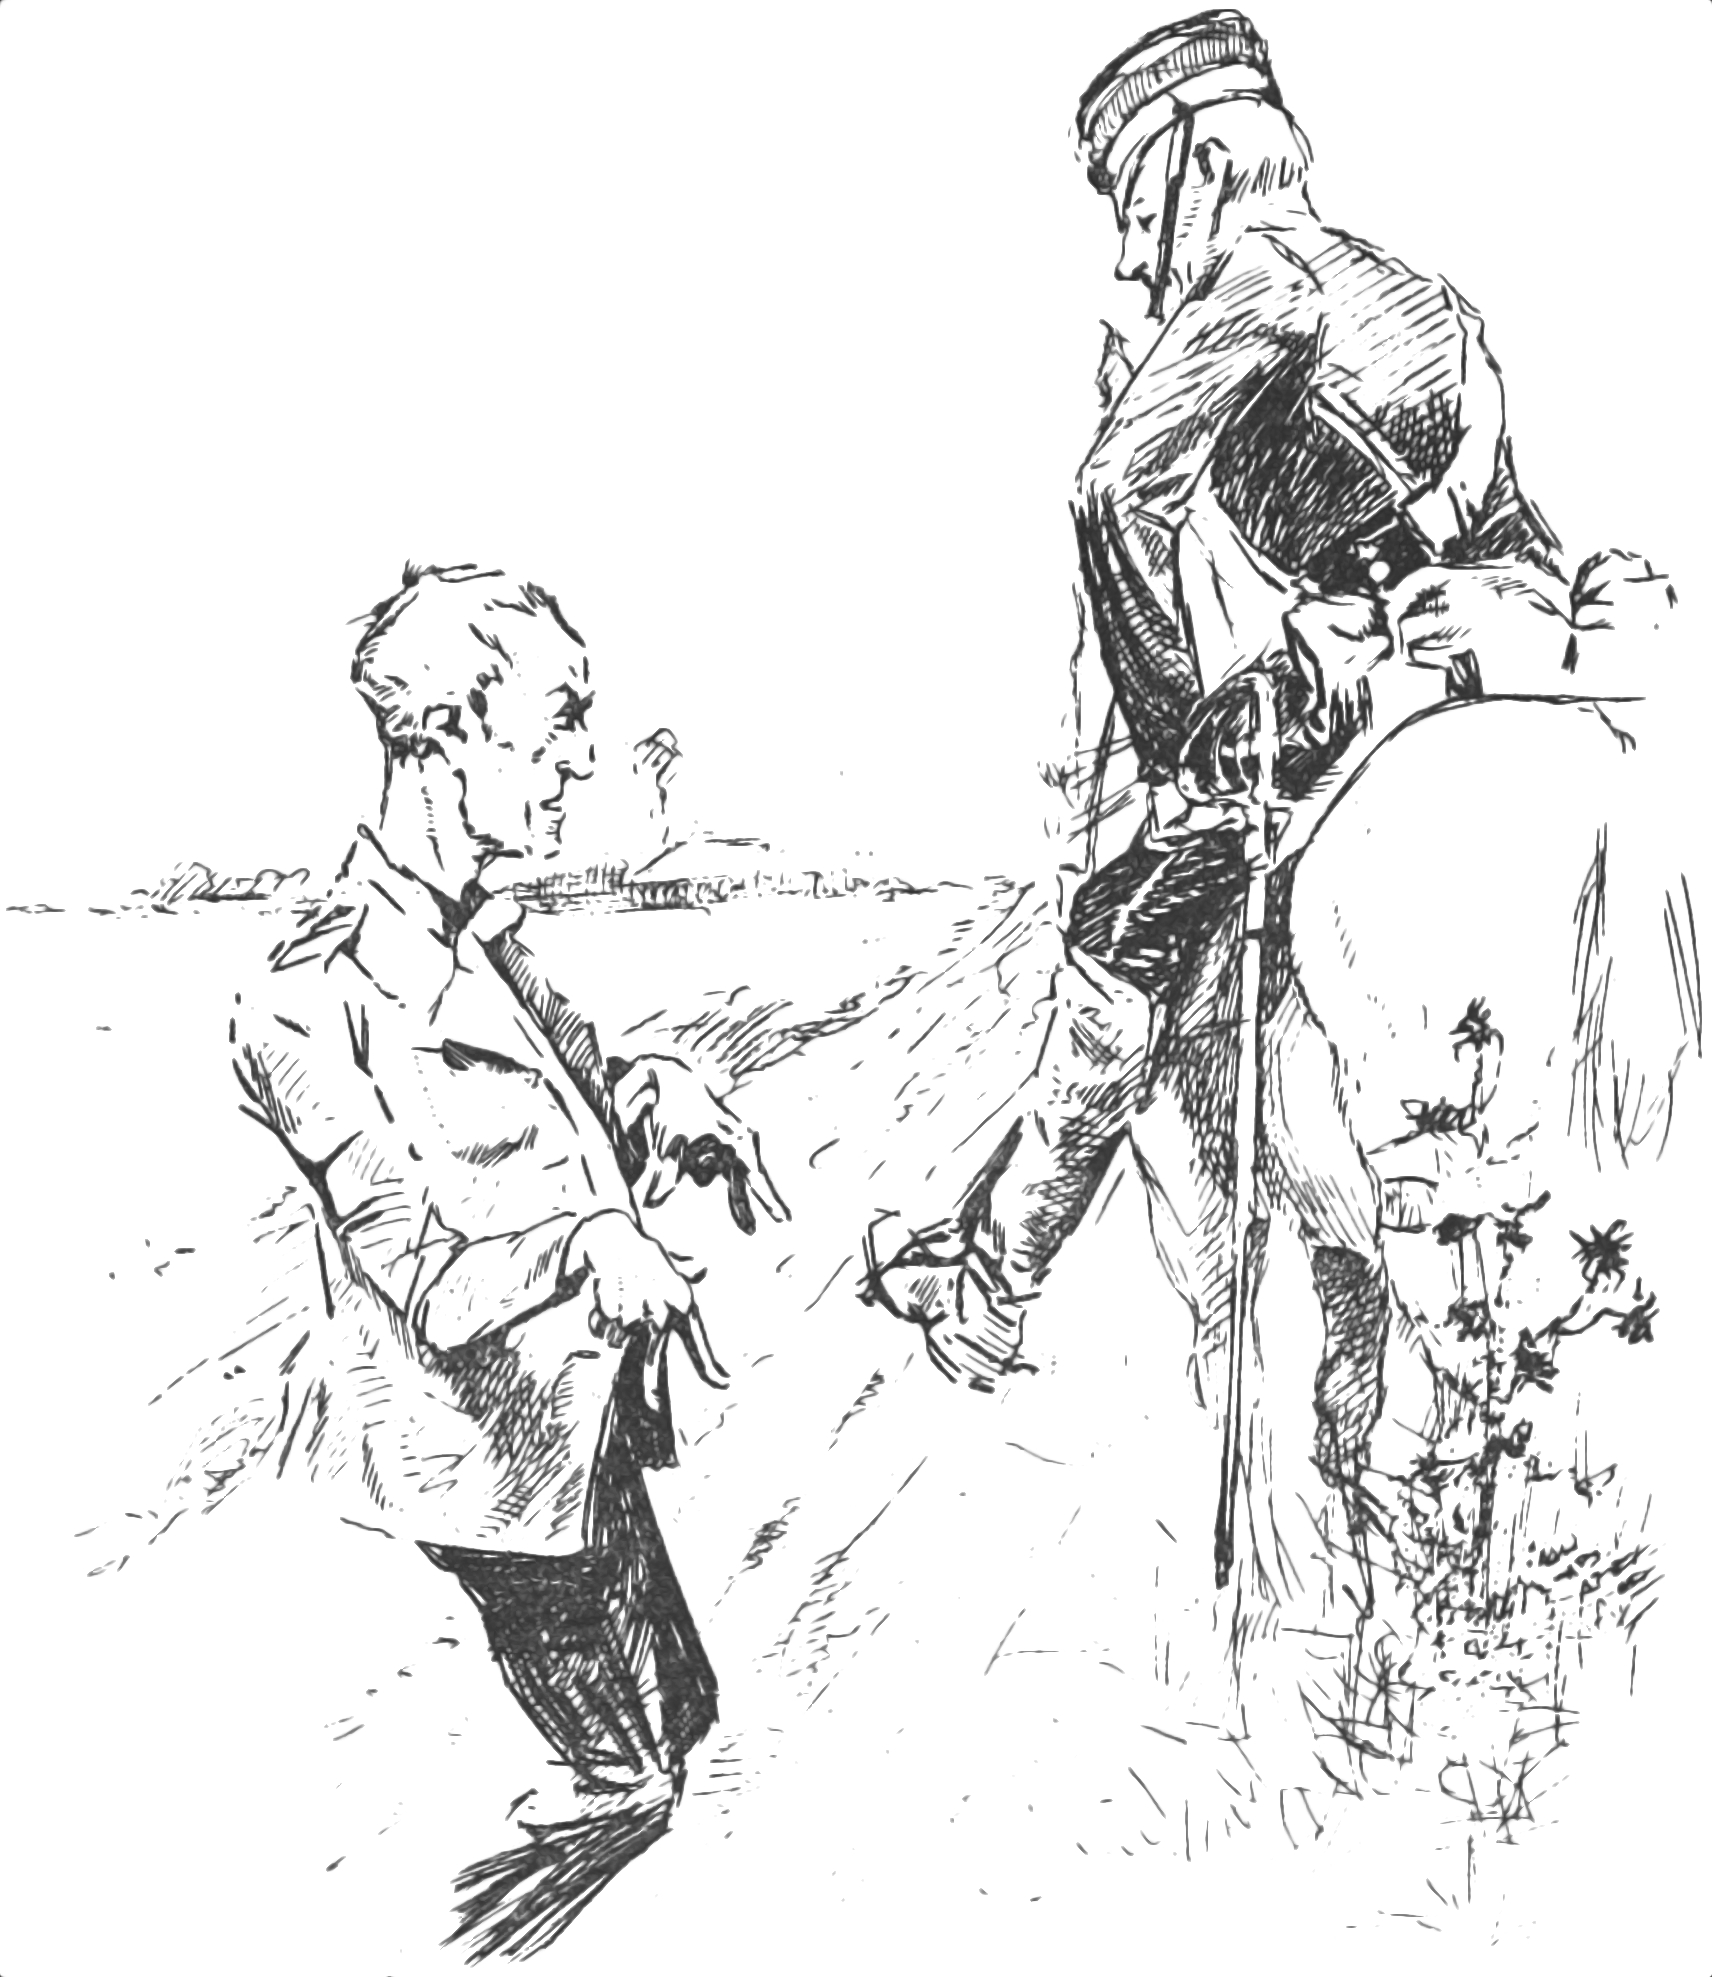
\includegraphics[width=0.5\textwidth]{12inspection}
\end{wrapfigure}
}{%

}
\makeatother

Farther along we came upon a group of three women and two children in the road, busy clearing out a labourer's cottage. They had got hold of a little hand truck, and were piling it up with unclean-looking bundles and shabby furniture. They were all too assiduously engaged to talk to us as we passed.

By Byfleet station we emerged from the pine trees, and found the country calm and peaceful under the morning sunlight. We were far beyond the range of the Heat-Ray there, and had it not been for the silent desertion of some of the houses, the stirring movement of packing in others, and the knot of soldiers standing on the bridge over the railway and staring down the line towards Woking, the day would have seemed very like any other Sunday.

Several farm waggons and carts were moving creakily along the road to Addlestone, and suddenly through the gate of a field we saw, across a stretch of flat meadow, six twelve-pounders standing neatly at equal distances pointing towards Woking. The gunners stood by the guns waiting, and the ammunition waggons were at a business-like distance. The men stood almost as if under inspection.

»That's good!« said I. »They will get one fair shot, at any rate.«

The artilleryman hesitated at the gate.

»I shall go on,« he said.

Farther on towards Weybridge, just over the bridge, there were a number of men in white fatigue jackets throwing up a long rampart, and more guns behind.

»It's bows and arrows against the lightning, anyhow,« said the artilleryman. »They `aven't seen that fire-beam yet.«

The officers who were not actively engaged stood and stared over the treetops southwestward, and the men digging would stop every now and again to stare in the same direction.


Byfleet was in a tumult; people packing, and a score of hussars, some of them dismounted, some on horseback, were hunting them about. Three or four black government waggons, with crosses in white circles, and an old omnibus, among other vehicles, were being loaded in the village street. There were scores of people, most of them sufficiently sabbatical to have assumed their best clothes. The soldiers were having the greatest difficulty in making them realise the gravity of their position. We saw one shrivelled old fellow with a huge box and a score or more of flower pots containing orchids, angrily expostulating with the corporal who would leave them behind. I stopped and gripped his arm.

»Do you know what's over there?« I said, pointing at the pine tops that hid the Martians.

»Eh?« said he, turning. »I was explainin' these is vallyble.«

»Death!« I shouted. »Death is coming! Death!« and leaving him to digest that if he could, I hurried on after the artillery-man. At the corner I looked back. The soldier had left him, and he was still standing by his box, with the pots of orchids on the lid of it, and staring vaguely over the trees.

\begin{wrapfigure}{O}{0.5\textwidth}
\centering

\includegraphics[width=0.5\textwidth]{12orchids}
\end{wrapfigure}

No one in Weybridge could tell us where the headquarters were established; the whole place was in such confusion as I had never seen in any town before. Carts, carriages everywhere, the most astonishing miscellany of conveyances and horseflesh. The respectable inhabitants of the place, men in golf and boating costumes, wives prettily dressed, were packing, river-side loafers energetically helping, children excited, and, for the most part, highly delighted at this astonishing variation of their Sunday experiences. In the midst of it all the worthy vicar was very pluckily holding an early celebration, and his bell was jangling out above the excitement.

I and the artilleryman, seated on the step of the drinking fountain, made a very passable meal upon what we had brought with us. Patrols of soldiers—here no longer hussars, but grenadiers in white—were warning people to move now or to take refuge in their cellars as soon as the firing began. We saw as we crossed the railway bridge that a growing crowd of people had assembled in and about the railway station, and the swarming platform was piled with boxes and packages. The ordinary traffic had been stopped, I believe, in order to allow of the passage of troops and guns to Chertsey, and I have heard since that a savage struggle occurred for places in the special trains that were put on at a later hour.

We remained at Weybridge until midday, and at that hour we found ourselves at the place near Shepperton Lock where the Wey and Thames join. Part of the time we spent helping two old women to pack a little cart. The Wey has a treble mouth, and at this point boats are to be hired, and there was a ferry across the river. On the Shepperton side was an inn with a lawn, and beyond that the tower of Shepperton Church—it has been replaced by a spire—rose above the trees.

\begin{wrapfigure}{O}{0.5\textwidth}
\centering
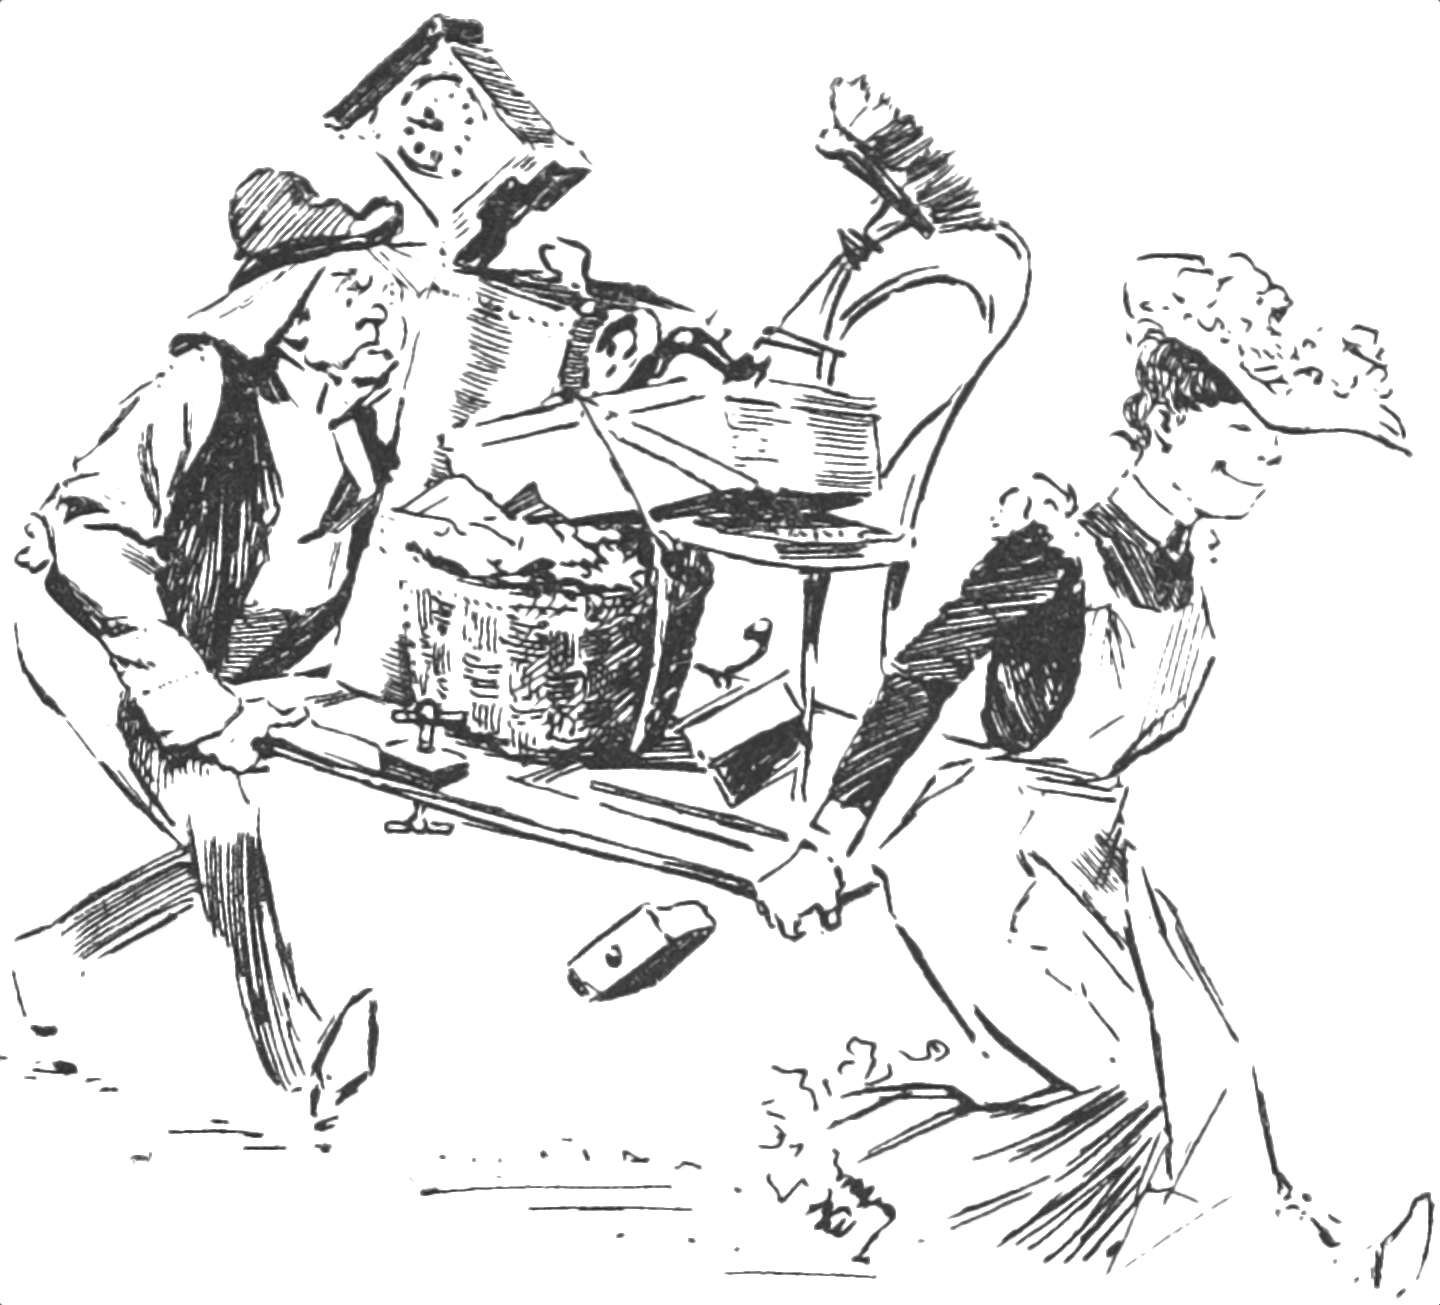
\includegraphics[width=0.5\textwidth]{12fugitives}
\end{wrapfigure}

Here we found an excited and noisy crowd of fugitives. As yet the flight had not grown to a panic, but there were already far more people than all the boats going to and fro could enable to cross. People came panting along under heavy burdens; one husband and wife were even carrying a small outhouse door between them, with some of their household goods piled thereon. One man told us he meant to try to get away from Shepperton station.

There was a lot of shouting, and one man was even jesting. The idea people seemed to have here was that the Martians were simply formidable human beings, who might attack and sack the town, to be certainly destroyed in the end. Every now and then people would glance nervously across the Wey, at the meadows towards Chertsey, but everything over there was still.

Across the Thames, except just where the boats landed, everything was quiet, in vivid contrast with the Surrey side. The people who landed there from the boats went tramping off down the lane. The big ferryboat had just made a journey. Three or four soldiers stood on the lawn of the inn, staring and jesting at the fugitives, without offering to help. The inn was closed, as it was now within prohibited hours.

»What's that?« cried a boatman, and »Shut up, you fool!« said a man near me to a yelping dog. Then the sound came again, this time from the direction of Chertsey, a muffled thud—the sound of a gun.

The fighting was beginning. Almost immediately unseen batteries across the river to our right, unseen because of the trees, took up the chorus, firing heavily one after the other. A woman screamed. Everyone stood arrested by the sudden stir of battle, near us and yet invisible to us. Nothing was to be seen save flat meadows, cows feeding unconcernedly for the most part, and silvery pollard willows motionless in the warm sunlight.

»The sojers'll stop `em,« said a woman beside me, doubtfully. A haziness rose over the treetops.

Then suddenly we saw a rush of smoke far away up the river, a puff of smoke that jerked up into the air and hung; and forthwith the ground heaved under foot and a heavy explosion shook the air, smashing two or three windows in the houses near, and leaving us astonished.

»Here they are!« shouted a man in a blue jersey. »Yonder! D'yer see them? Yonder!«

Quickly, one after the other, one, two, three, four of the armoured Martians appeared, far away over the little trees, across the flat meadows that stretched towards Chertsey, and striding hurriedly towards the river. Little cowled figures they seemed at first, going with a rolling motion and as fast as flying birds.

Then, advancing obliquely towards us, came a fifth. Their armoured bodies glittered in the sun as they swept swiftly forward upon the guns, growing rapidly larger as they drew nearer. One on the extreme left, the remotest that is, flourished a huge case high in the air, and the ghostly, terrible Heat-Ray I had already seen on Friday night smote towards Chertsey, and struck the town.

At sight of these strange, swift, and terrible creatures the crowd near the water's edge seemed to me to be for a moment horror-struck. There was no screaming or shouting, but a silence. Then a hoarse murmur and a movement of feet—a splashing from the water. A man, too frightened to drop the portmanteau he carried on his shoulder, swung round and sent me staggering with a blow from the corner of his burden. A woman thrust at me with her hand and rushed past me. I turned with the rush of the people, but I was not too terrified for thought. The terrible Heat-Ray was in my mind. To get under water! That was it!

»Get under water!« I shouted, unheeded.

I faced about again, and rushed towards the approaching Martian, rushed right down the gravelly beach and headlong into the water. Others did the same. A boatload of people putting back came leaping out as I rushed past. The stones under my feet were muddy and slippery, and the river was so low that I ran perhaps twenty feet scarcely waist-deep. Then, as the Martian towered overhead scarcely a couple of hundred yards away, I flung myself forward under the surface. The splashes of the people in the boats leaping into the river sounded like thunderclaps in my ears. People were landing hastily on both sides of the river. But the Martian machine took no more notice for the moment of the people running this way and that than a man would of the confusion of ants in a nest against which his foot has kicked. When, half suffocated, I raised my head above water, the Martian's hood pointed at the batteries that were still firing across the river, and as it advanced it swung loose what must have been the generator of the Heat-Ray.

In another moment it was on the bank, and in a stride wading halfway across. The knees of its foremost legs bent at the farther bank, and in another moment it had raised itself to its full height again, close to the village of Shepperton. Forthwith the six guns which, unknown to anyone on the right bank, had been hidden behind the outskirts of that village, fired simultaneously. The sudden near concussion, the last close upon the first, made my heart jump. The monster was already raising the case generating the Heat-Ray as the first shell burst six yards above the hood.

I gave a cry of astonishment. I saw and thought nothing of the other four Martian monsters; my attention was riveted upon the nearer incident. Simultaneously two other shells burst in the air near the body as the hood twisted round in time to receive, but not in time to dodge, the fourth shell.

\begin{figure}[tbp]
\centering

\includegraphics[width=\linewidth]{12fourthshell}
\caption{»Hit!« shouted I}
\end{figure}

The shell burst clean in the face of the Thing. The hood bulged, flashed, was whirled off in a dozen tattered fragments of red flesh and glittering metal.

»Hit!« shouted I, with something between a scream and a cheer.

I heard answering shouts from the people in the water about me. I could have leaped out of the water with that momentary exultation.

The decapitated colossus reeled like a drunken giant; but it did not fall over. It recovered its balance by a miracle, and, no longer heeding its steps and with the camera that fired the Heat-Ray now rigidly upheld, it reeled swiftly upon Shepperton. The living intelligence, the Martian within the hood, was slain and splashed to the four winds of heaven, and the Thing was now but a mere intricate device of metal whirling to destruction. It drove along in a straight line, incapable of guidance. It struck the tower of Shepperton Church, smashing it down as the impact of a battering ram might have done, swerved aside, blundered on and collapsed with tremendous force into the river out of my sight.

A violent explosion shook the air, and a spout of water, steam, mud, and shattered metal shot far up into the sky. As the camera of the Heat-Ray hit the water, the latter had immediately flashed into steam. In another moment a huge wave, like a muddy tidal bore but almost scaldingly hot, came sweeping round the bend upstream. I saw people struggling shorewards, and heard their screaming and shouting faintly above the seething and roar of the Martian's collapse.

For a moment I heeded nothing of the heat, forgot the patent need of self-preservation. I splashed through the tumultuous water, pushing aside a man in black to do so, until I could see round the bend. Half a dozen deserted boats pitched aimlessly upon the confusion of the waves. The fallen Martian came into sight downstream, lying across the river, and for the most part submerged.

Thick clouds of steam were pouring off the wreckage, and through the tumultuously whirling wisps I could see, intermittently and vaguely, the gigantic limbs churning the water and flinging a splash and spray of mud and froth into the air. The tentacles swayed and struck like living arms, and, save for the helpless purposelessness of these movements, it was as if some wounded thing were struggling for its life amid the waves. Enormous quantities of a ruddy-brown fluid were spurting up in noisy jets out of the machine.

My attention was diverted from this death flurry by a furious yelling, like that of the thing called a siren in our manufacturing towns. A man, knee-deep near the towing path, shouted inaudibly to me and pointed. Looking back, I saw the other Martians advancing with gigantic strides down the riverbank from the direction of Chertsey. The Shepperton guns spoke this time unavailingly.

At that I ducked at once under water, and, holding my breath until movement was an agony, blundered painfully ahead under the surface as long as I could. The water was in a tumult about me, and rapidly growing hotter.

When for a moment I raised my head to take breath and throw the hair and water from my eyes, the steam was rising in a whirling white fog that at first hid the Martians altogether. The noise was deafening. Then I saw them dimly, colossal figures of grey, magnified by the mist. They had passed by me, and two were stooping over the frothing, tumultuous ruins of their comrade.

The third and fourth stood beside him in the water, one perhaps two hundred yards from me, the other towards Laleham. The generators of the Heat-Rays waved high, and the hissing beams smote down this way and that.


\begin{figure}[tbp]
\centering
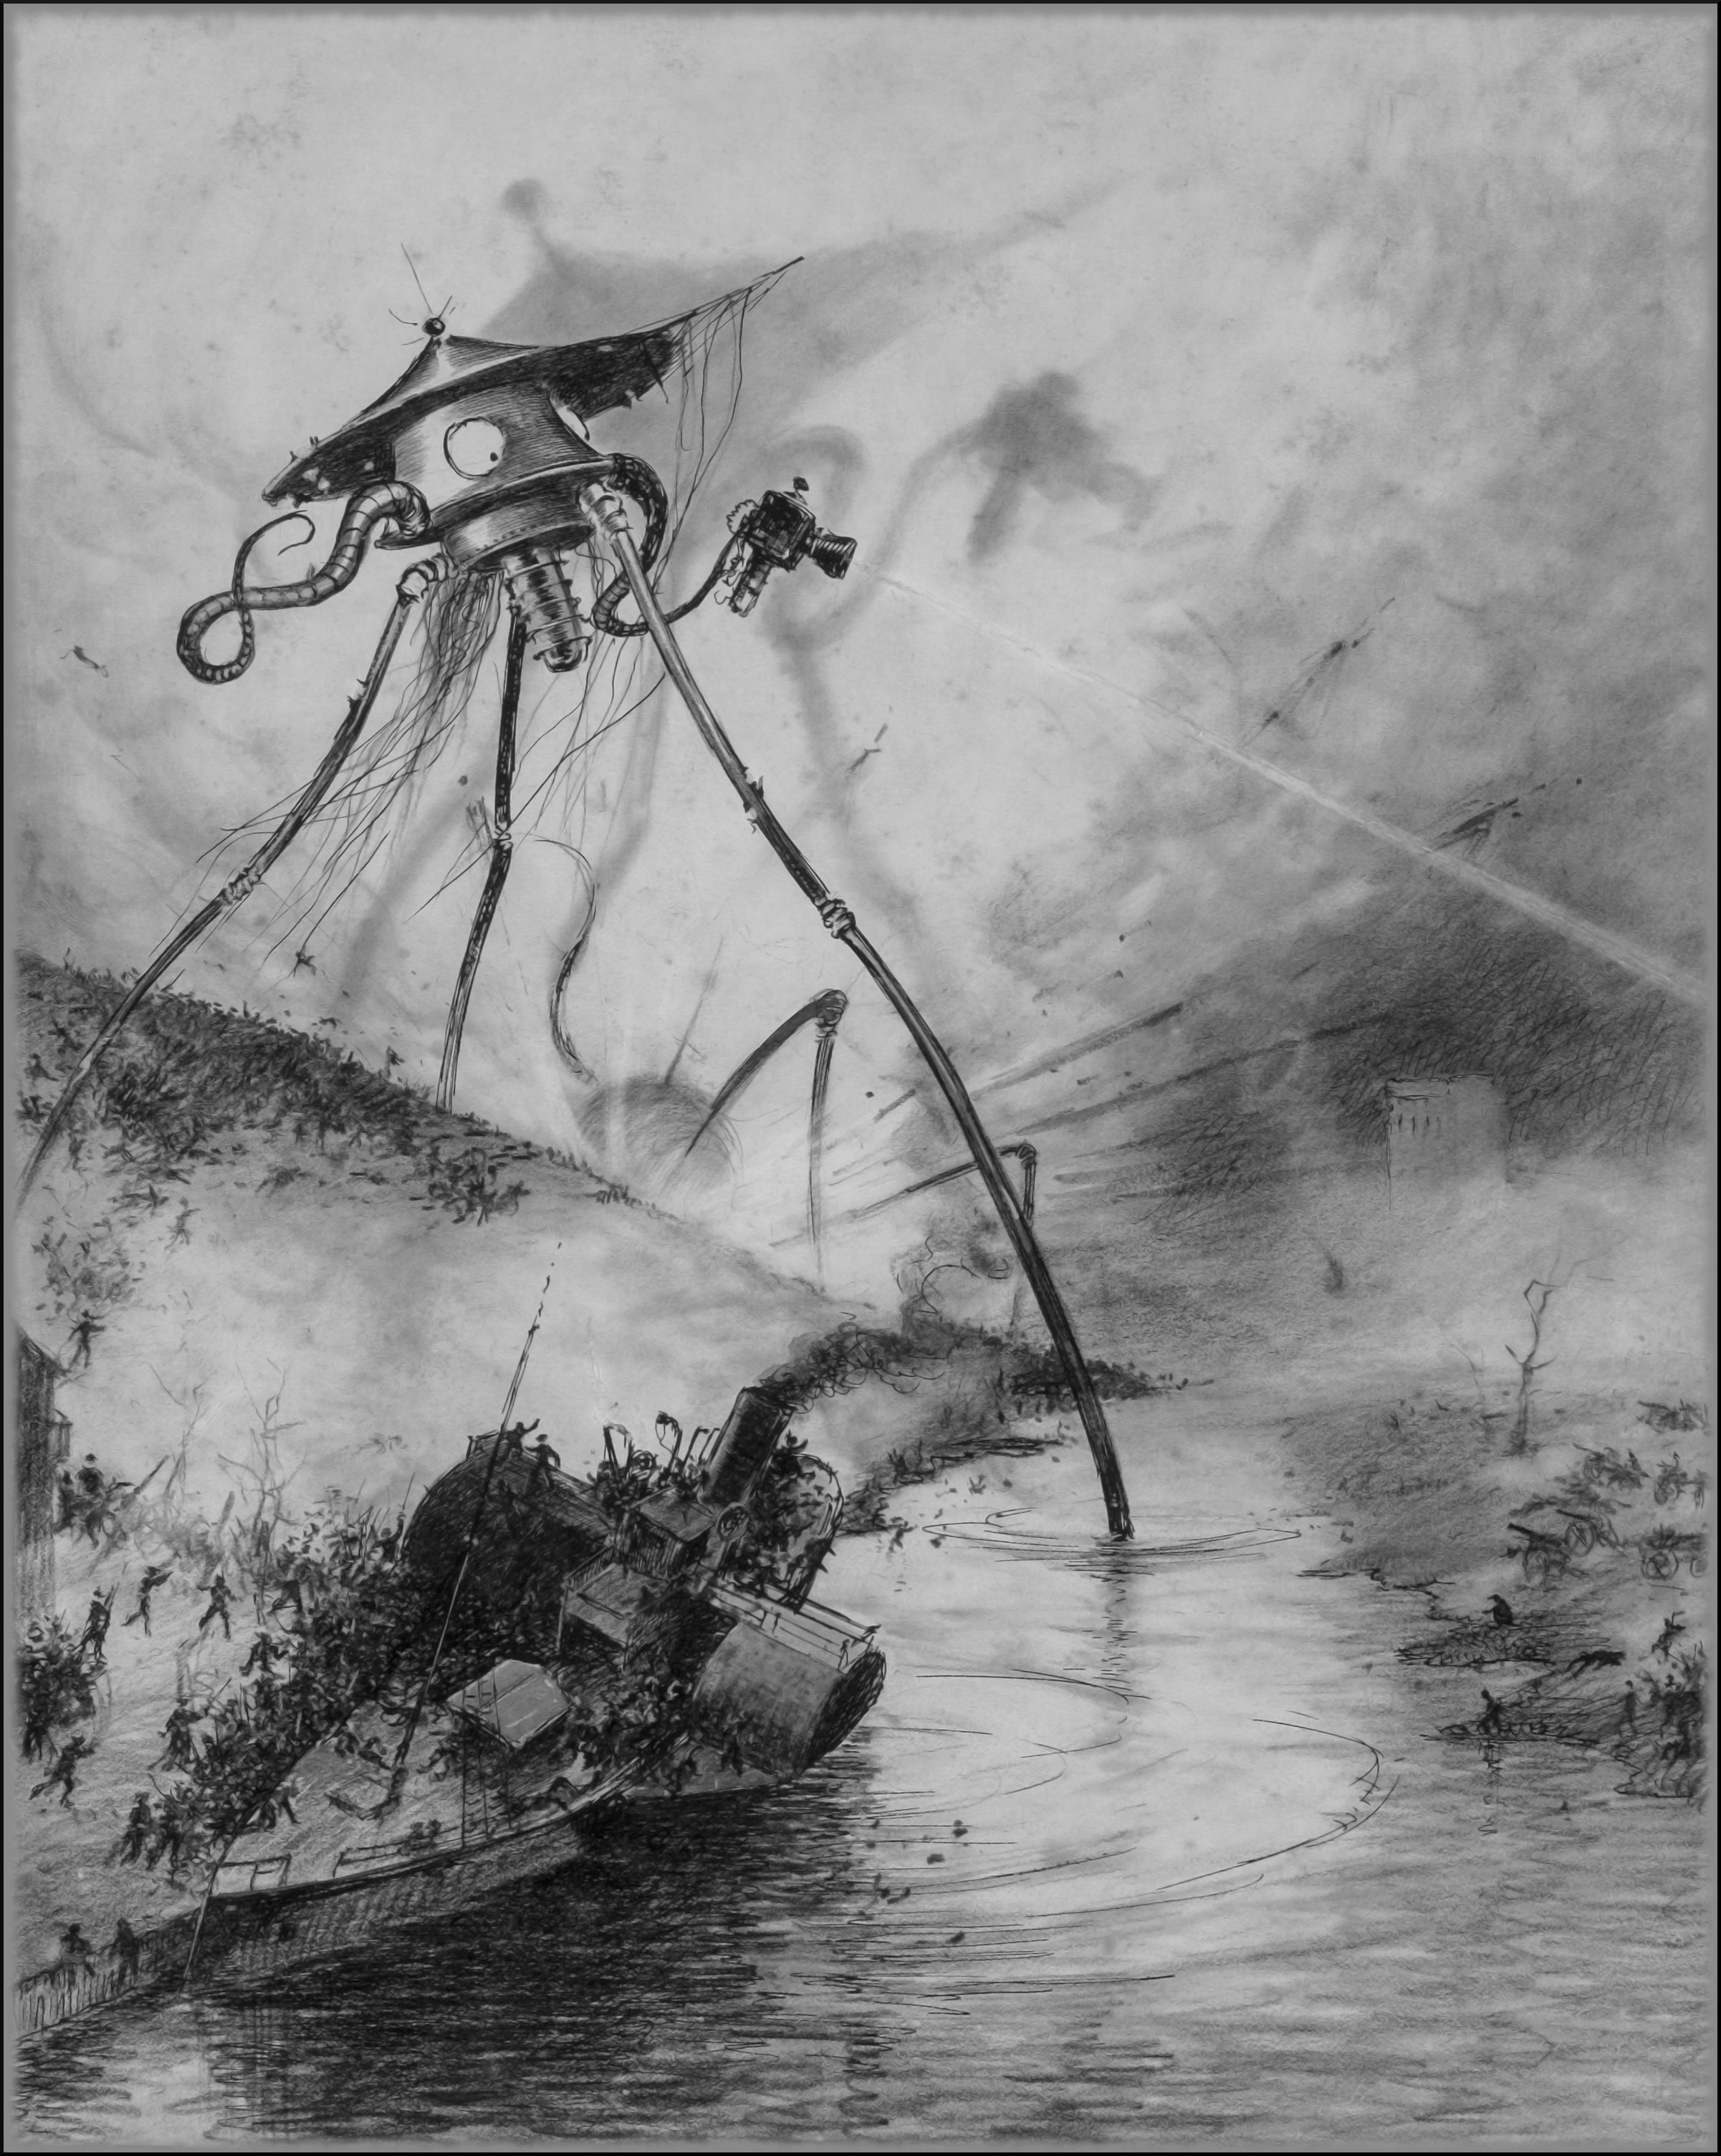
\includegraphics[width=\linewidth]{12besidehim}
\caption{The hissing beams smote down this way and that}
\end{figure}

The air was full of sound, a deafening and confusing conflict of noises—the clangorous din of the Martians, the crash of falling houses, the thud of trees, fences, sheds flashing into flame, and the crackling and roaring of fire. Dense black smoke was leaping up to mingle with the steam from the river, and as the Heat-Ray went to and fro over Weybridge its impact was marked by flashes of incandescent white, that gave place at once to a smoky dance of lurid flames. The nearer houses still stood intact, awaiting their fate, shadowy, faint and pallid in the steam, with the fire behind them going to and fro.

For a moment perhaps I stood there, breast-high in the almost boiling water, dumbfounded at my position, hopeless of escape. Through the reek I could see the people who had been with me in the river scrambling out of the water through the reeds, like little frogs hurrying through grass from the advance of a man, or running to and fro in utter dismay on the towing path.

Then suddenly the white flashes of the Heat-Ray came leaping towards me. The houses caved in as they dissolved at its touch, and darted out flames; the trees changed to fire with a roar. The Ray flickered up and down the towing path, licking off the people who ran this way and that, and came down to the water's edge not fifty yards from where I stood. It swept across the river to Shepperton, and the water in its track rose in a boiling weal crested with steam. I turned shoreward.

In another moment the huge wave, well-nigh at the boiling-point had rushed upon me. I screamed aloud, and scalded, half blinded, agonised, I staggered through the leaping, hissing water towards the shore. Had my foot stumbled, it would have been the end. I fell helplessly, in full sight of the Martians, upon the broad, bare gravelly spit that runs down to mark the angle of the Wey and Thames. I expected nothing but death.

I have a dim memory of the foot of a Martian coming down within a score of yards of my head, driving straight into the loose gravel, whirling it this way and that and lifting again; of a long suspense, and then of the four carrying the debris of their comrade between them, now clear and then presently faint through a veil of smoke, receding interminably, as it seemed to me, across a vast space of river and meadow. And then, very slowly, I realised that by a miracle I had escaped.

\begin{figure}[b!]
\centering
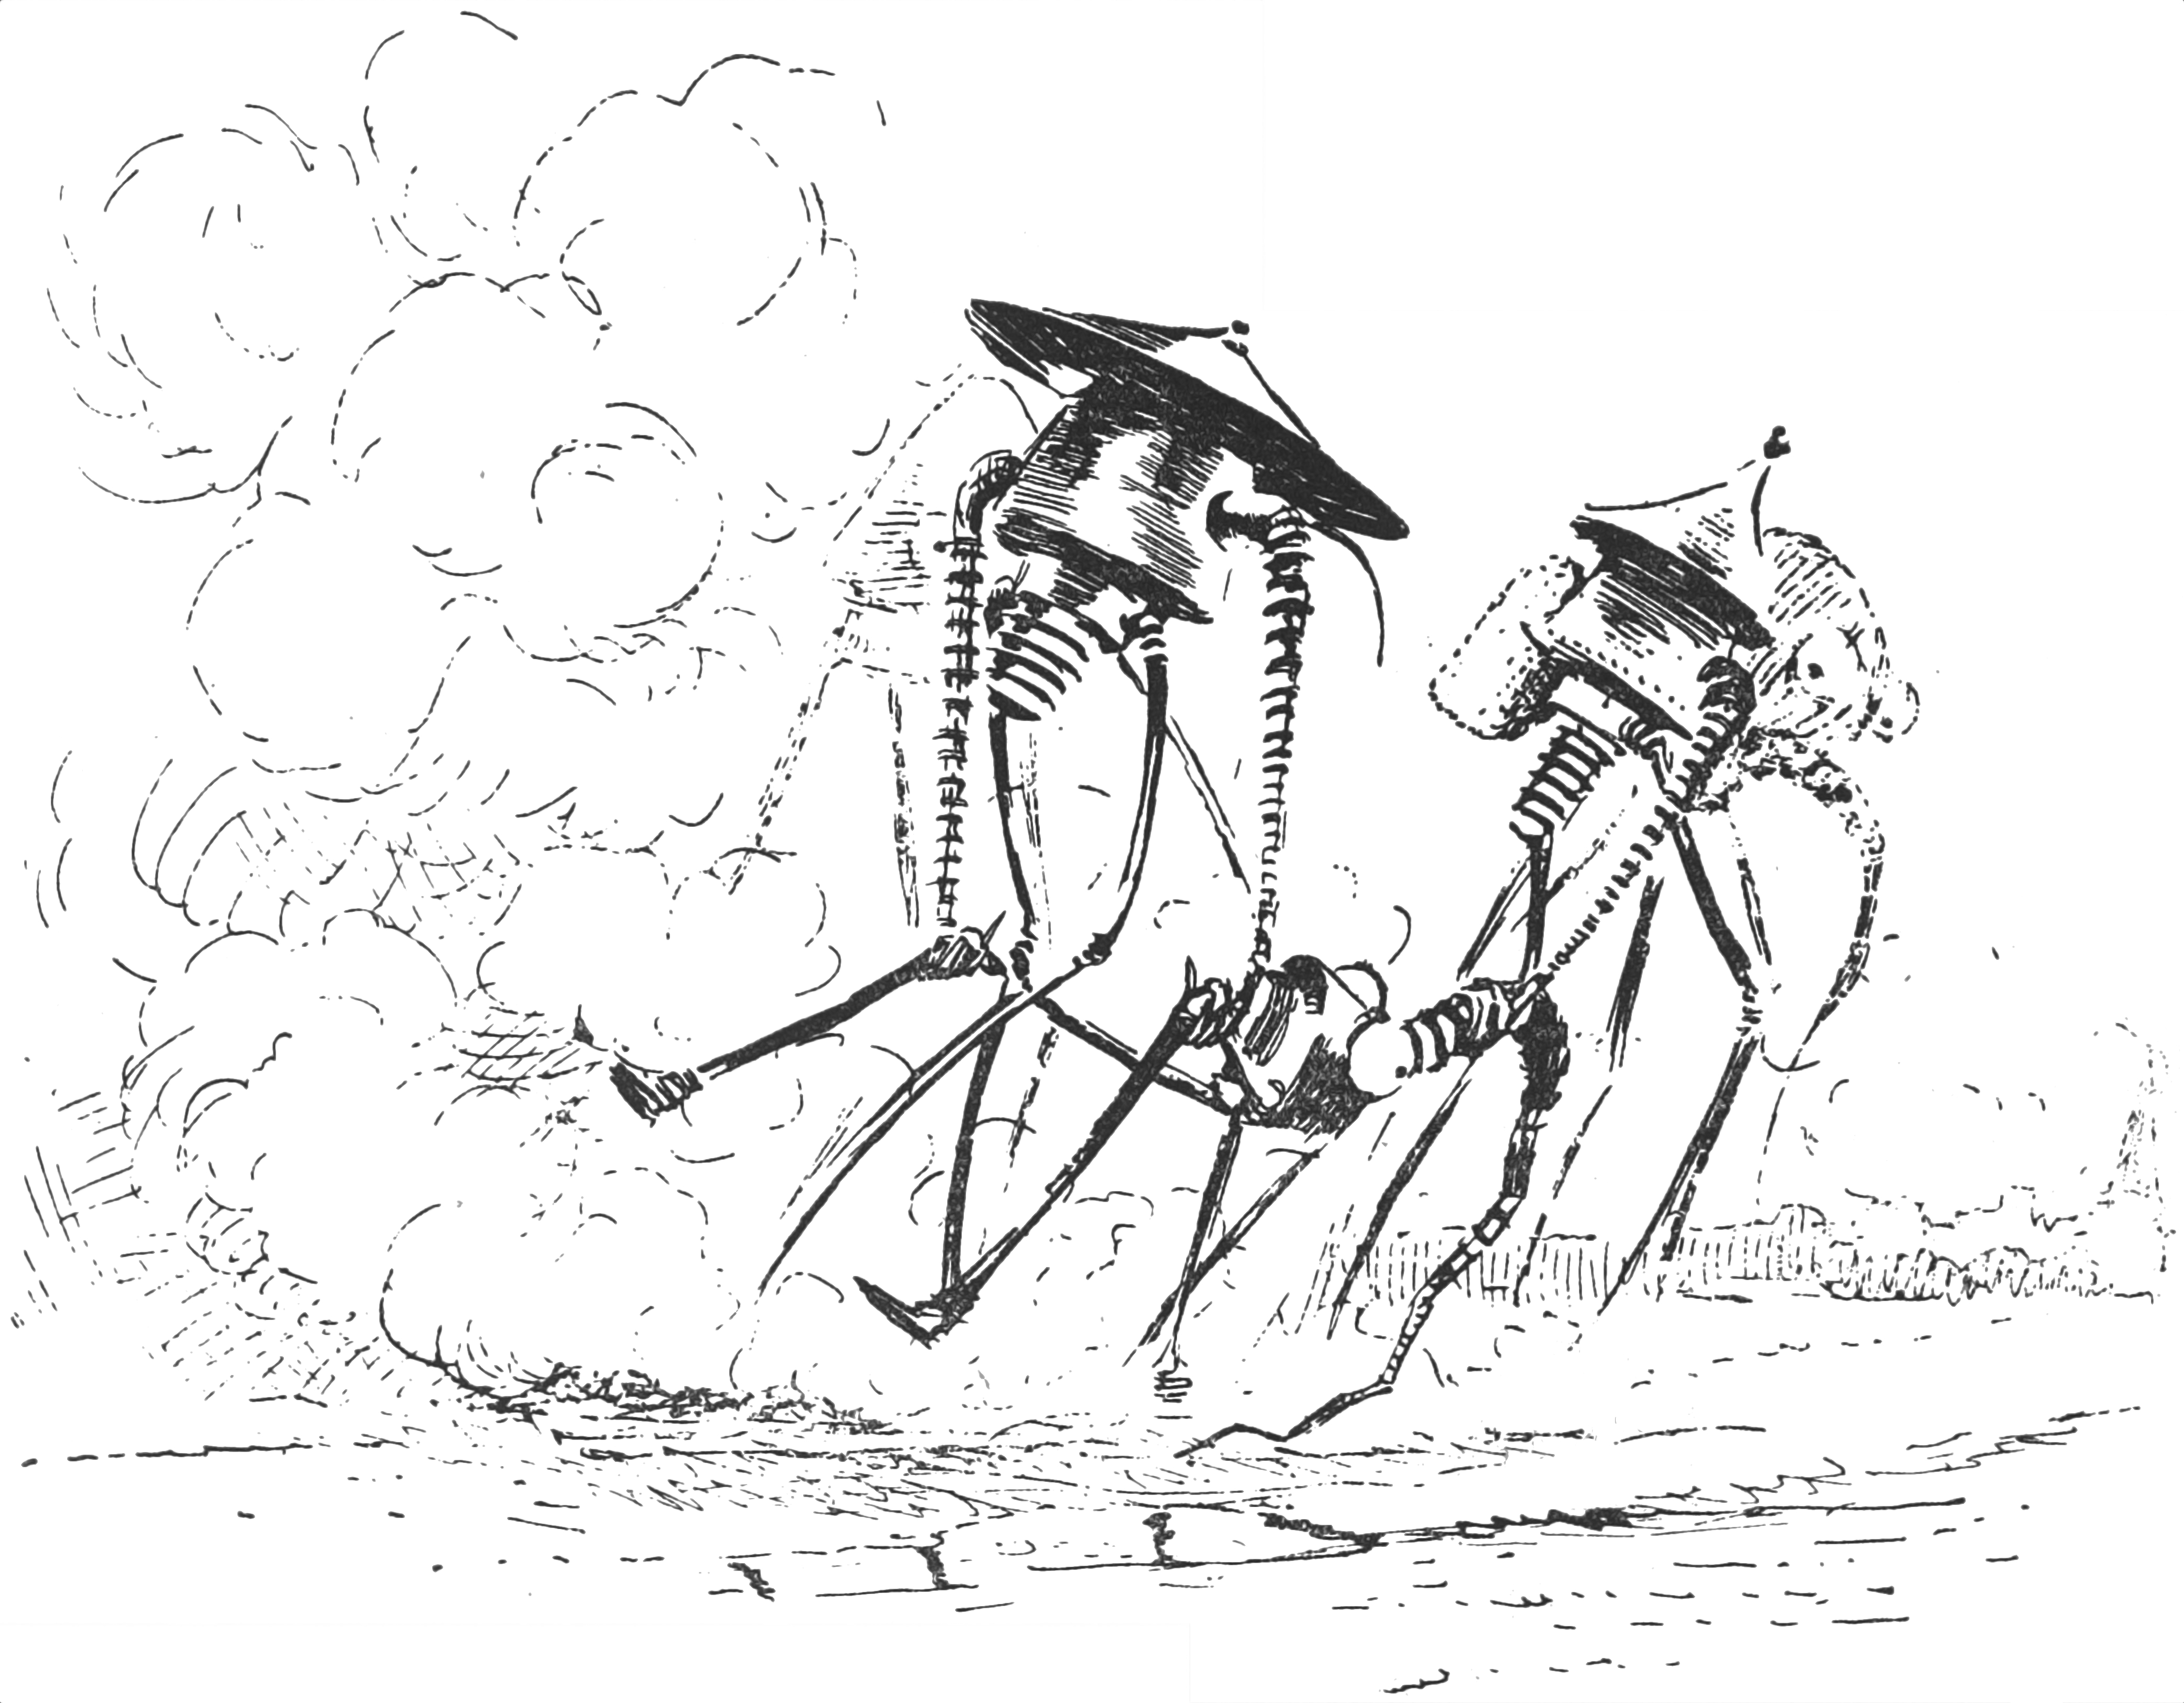
\includegraphics[width=\tailpiecesize]{12tailpiece}
%\captionlistentry{Tailpiece to Chapter \thechapter}
\end{figure}